\section{\textit{Service}}

\textit{Service} dapat diartikan sebagai sebuah teknologi atau cara kerja yang dapat digunakan untuk memberikan keuntungan ataupun menyelesaikan suatu pekerjaan. Selain itu \textit{service} juga dapat diartikan sebagai abstraksi dari sebuah proses bisnis. \parencite{osullivan2002}

Secara umum \textit{Service} Memiliki tiga fitur utama yaitu.
\begin{enumerate}
  \item \textit{Service} dapat melakukan sebuah aksi atau pekerjaan untuk orang lain,
  \item \textit{Service} adalah sebuah aset yang memiliki sebuah nilai yang dapat diturunkan dari penyedia ke pengguna,
  \item \textit{Service} dapat di bungkus pada service lainnya (sub-services),
\end{enumerate}

Untuk menggabungkan \textit{service}, terdapat dua cara yaitu agregasi dan komposisi. Agregasi memiliki pendekatan untuk menggabungkan dua atau lebih \textit{service} dan membuat satu \textit{entrypoint} untuk seluruh \textit{service} tersebut. Berbeda dengan komposisi, komposisi menggunakan pendekatan untuk mengintegrasikan seluruh sub-\textit{services} yang ada dengan cara membuat jalur komunikasi antar \textit{service} dan setiap \textit{service} memiliki hubungan tertentu dengan \textit{service} lainnya.

Interaksi pada sebuah \textit{service} haruslah minimal memiliki tiga elemen, \textit{service provider}, \textit{service requestor/client}, serta \textit{\textit{service registry}}, namun terdapat juga elemen ke empat pada beberapa kasus yaitu \textit{service broker}. Illustrasi dapat dilhat pada gambar \ref{fig:tiga-elemen-service}

\begin{figure}[ht]
  \centering
  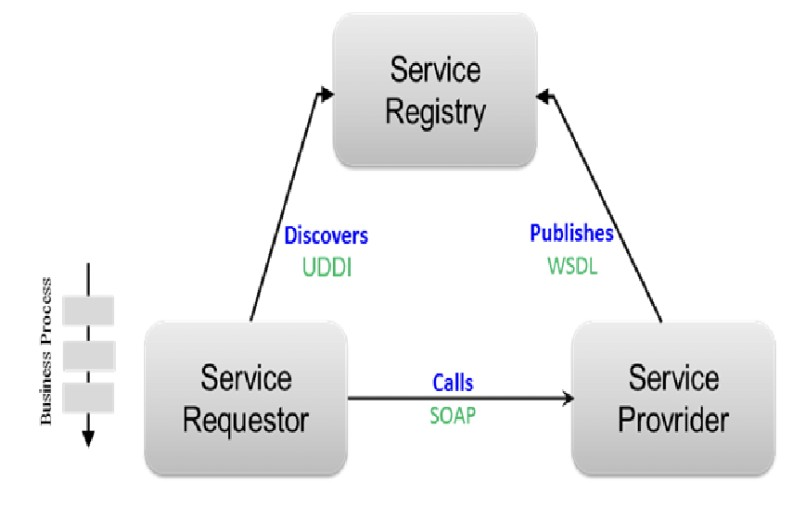
\includegraphics[width=0.8\textwidth]{chapter-2/tiga-elemen-service.jpg}
  \caption{Tiga Elemen pada Interaksi Service, \parencite{abugessaisa2023}}
  \label{fig:tiga-elemen-service}
\end{figure}

\textit{Service requestor} mengirimkan permintaannya serta kebutuhannya kepada \textit{service registry} untuk dicarikan service yang sesuai dengan kebutuhannya. Namun pada beberapa kasus khusus, \textit{service requestor}
sudah memiliki \textquotedblleft contract \textquotedblright dengan \textit{provider} tujuannya sehingga bisa langsung melakukan \textit{request} ke \textit{provider} tanpa bantuan dari \textit{service registry}.

Service \textit{provider} menyediakan \textit{service} yang dapat dikonsumsi oleh publik, agar \textit{service} nya dapat digunakan oleh requestor, \textit{service} \textit{provider} akan memberikan list \textit{services} yang dimiliki kepada registry untuk disimpan pada sebuah \textquotedblleft catalogue \textquotedblright yang dimiliki oleh registry.\textit{Service registry} berperan sebagai penengah dalam komunikasi \textit{requestor} dan \textit{provider}. \textit{Service registry} memiliki \textquotedblleft catalogue \textquotedblright yang menyimpan list berbagai macam \textit{service provider} yang dapat digunakan oleh \textit{service requestor}.

Dengan adanya ketiga elemen tersebut, interaksi pada \textit{services} dapat berjalan sehingga menciptakan suatu fungsionalitas seperti proses bisnis ataupun pemenuhan kebutuhan lainnya.
